\documentclass[]{article}
\usepackage{lmodern}
\usepackage{amssymb,amsmath}
\usepackage{ifxetex,ifluatex}
\usepackage{fixltx2e} % provides \textsubscript
\ifnum 0\ifxetex 1\fi\ifluatex 1\fi=0 % if pdftex
  \usepackage[T1]{fontenc}
  \usepackage[utf8]{inputenc}
\else % if luatex or xelatex
  \ifxetex
    \usepackage{mathspec}
  \else
    \usepackage{fontspec}
  \fi
  \defaultfontfeatures{Ligatures=TeX,Scale=MatchLowercase}
\fi
% use upquote if available, for straight quotes in verbatim environments
\IfFileExists{upquote.sty}{\usepackage{upquote}}{}
% use microtype if available
\IfFileExists{microtype.sty}{%
\usepackage[]{microtype}
\UseMicrotypeSet[protrusion]{basicmath} % disable protrusion for tt fonts
}{}
\PassOptionsToPackage{hyphens}{url} % url is loaded by hyperref
\usepackage[unicode=true]{hyperref}
\hypersetup{
            pdftitle={Results},
            pdfborder={0 0 0},
            breaklinks=true}
\urlstyle{same}  % don't use monospace font for urls
\usepackage[margin=1in]{geometry}
\usepackage{graphicx,grffile}
\makeatletter
\def\maxwidth{\ifdim\Gin@nat@width>\linewidth\linewidth\else\Gin@nat@width\fi}
\def\maxheight{\ifdim\Gin@nat@height>\textheight\textheight\else\Gin@nat@height\fi}
\makeatother
% Scale images if necessary, so that they will not overflow the page
% margins by default, and it is still possible to overwrite the defaults
% using explicit options in \includegraphics[width, height, ...]{}
\setkeys{Gin}{width=\maxwidth,height=\maxheight,keepaspectratio}
\IfFileExists{parskip.sty}{%
\usepackage{parskip}
}{% else
\setlength{\parindent}{0pt}
\setlength{\parskip}{6pt plus 2pt minus 1pt}
}
\setlength{\emergencystretch}{3em}  % prevent overfull lines
\providecommand{\tightlist}{%
  \setlength{\itemsep}{0pt}\setlength{\parskip}{0pt}}
\setcounter{secnumdepth}{0}
% Redefines (sub)paragraphs to behave more like sections
\ifx\paragraph\undefined\else
\let\oldparagraph\paragraph
\renewcommand{\paragraph}[1]{\oldparagraph{#1}\mbox{}}
\fi
\ifx\subparagraph\undefined\else
\let\oldsubparagraph\subparagraph
\renewcommand{\subparagraph}[1]{\oldsubparagraph{#1}\mbox{}}
\fi

% set default figure placement to htbp
\makeatletter
\def\fps@figure{htbp}
\makeatother

\usepackage{booktabs}
\usepackage{longtable}
\usepackage{array}
\usepackage{multirow}
\usepackage{wrapfig}
\usepackage{float}
\usepackage{colortbl}
\usepackage{pdflscape}
\usepackage{tabu}
\usepackage{threeparttable}
\usepackage{threeparttablex}
\usepackage[normalem]{ulem}
\usepackage{makecell}
\usepackage{xcolor}

\title{Results}
\author{}
\date{\vspace{-2.5em}}

\begin{document}
\maketitle

An introduction to results. A description of each one of the results.

\subsubsection{Participants}\label{participants}

\begin{table}

\caption{\label{tab:unnamed-chunk-1}Participants demographics}
\centering
\begin{tabular}[t]{l|l|l|l|l|l|l|l|l|l}
\hline
participant & gender & age & occupation & country of origin & type accomodation & people in accomodation & inhabitants in accomodation & first session & helpers\\
\hline
\rowcolor{gray!6}  1 & male & 25 & PhD student & Indonesia & house & 2 & professionals & reg & \\
\hline
2 & non binary & 28 & PhD student & Germany & house & 4 & students & new & \\
\hline
\rowcolor{gray!6}  3 & male & 19 & Undergraduate student & Hong Kong & flat & 6 & students & reg & \\
\hline
4 & female & 50 & Impact officer & USA & house & 4 & family & new & \\
\hline
\rowcolor{gray!6}  5 & male & 30 & Administrator & UK & house & 2 & couple & reg & new\\
\hline
6 & female & 32 & Jobseeker & Hong Kong & house & 4 & professionals & reg & \\
\hline
\rowcolor{gray!6}  7 & male & 32 & PhD student & Iraq & flat & 3 & family & reg & \\
\hline
8 & female & 33 & PhD student & Russia & flat & 1 & individual & reg & \\
\hline
\rowcolor{gray!6}  9 & female & 29 & Invigilator & Mexico & flat & 2 & couple & new & reg \& new\\
\hline
10 & male & 29 & PhD student & Greece & flat & 2 & couple & reg & \\
\hline
\rowcolor{gray!6}  11 & female & 29 & PhD student & Bosnia and Herzegovina & flat & 2 & couple & new & \\
\hline
12 & male & 46 & Researcher & Mexico & house & 5 & family & reg & \\
\hline
\rowcolor{gray!6}  13 & female & 29 & Lecturer & UK & house & 2 & couple & new & new\\
\hline
14 & female & 35 & Housewife & Mexico & house & 4 & family & new & \\
\hline
\rowcolor{gray!6}  15 & female & 72 & Retired & Puerto Rico & house & 2 & couple & new & \\
\hline
16 & female & 40 & Housewife & Mexico & house & 3 & family & reg & \\
\hline
\rowcolor{gray!6}  17 & female & 32 & Research fellow & Ireland & house & 6 & professionals & reg & \\
\hline
18 & female & 26 & Food scientist & UK & house & 3 & professionals & new & reg \& new\\
\hline
\rowcolor{gray!6}  19 & female & 37 & Supply chain manager & China & house & 3 & family & new & \\
\hline
20 & female & 46 & School director & UK & house & 3 & family & reg & \\
\hline
\end{tabular}
\end{table}

\subsubsection{Recipes}\label{recipes}

Add recipe source

\begin{table}

\caption{\label{tab:unnamed-chunk-2}List of recipes}
\centering
\begin{tabular}[t]{l|l|l}
\hline
session & regular & new\\
\hline
\rowcolor{gray!6}  1 & chicken coconut curry & mac and cheese\\
\hline
2 & chickpeas curry with rice & butternut squash curry with coconut milk\\
\hline
\rowcolor{gray!6}  3 & pasta bolognesa & stir fry chicken, rice and peas\\
\hline
4 & green vegs soup & creamy tomato and chorizo rigatoni\\
\hline
\rowcolor{gray!6}  5 & pasta bolognesa & mexican chicken stew\\
\hline
6 & noddles with vegetables (spaggetti) & chicken gyros\\
\hline
\rowcolor{gray!6}  7 & oven roasted chicken & pomegranate rice and salad\\
\hline
8 & scrambled eggs with vegs & ricotta pancakes\\
\hline
\rowcolor{gray!6}  9 & chicken fajitas with rice and fried beans & beef, bean, and beer chili\\
\hline
10 & scrambled eggs with vegs and sausages & mushroom risotto\\
\hline
\rowcolor{gray!6}  11 & pasta bolognesa with vegs & crispy five-spice chicken\\
\hline
12 & minced vegs with vegetables tacos & spanish tortilla (potatoes omelette)\\
\hline
\rowcolor{gray!6}  13 & creamy risssoto with vegs and prawns & keralan chicken curry\\
\hline
14 & vegetable-based stew & cream of spinach soup\\
\hline
\rowcolor{gray!6}  15 & rice with chickpeas (puerto rican rice) & spinach and chickpea soup\\
\hline
16 & roasted chicken and roasted vegetables & white beans with artichokes\\
\hline
\rowcolor{gray!6}  17 & shepherd's pie & szechuan cabbage and crispy chilli beef\\
\hline
18 & pasta carbonara \& pasta napolitana & malfatti ricotta and spinach \& hummus\\
\hline
\rowcolor{gray!6}  19 & shepherd's pie & prawn and black beans curry\\
\hline
20 & creamy chicken pasta & spicy beef with coriander relish\\
\hline
\end{tabular}
\end{table}

\subsubsection{Source of recipes}\label{source-of-recipes}

Description of the recipe source

\begin{table}

\caption{\label{tab:unnamed-chunk-3}Source of recipes}
\centering
\begin{tabular}[t]{l|l|l|l|l}
\hline
session & instrument & tool & source & duration\\
\hline
\rowcolor{gray!6}  1 & laptop & website & epicurious.com & 70\\
\hline
2 & phone & website & shefskitchen.com & \\
\hline
\rowcolor{gray!6}  3 & phone & website & studenthut.com & \\
\hline
4 & phone & website & kitchensanctuary.com & 25\\
\hline
\rowcolor{gray!6}  5 & phone & website & bbc.com & 45\\
\hline
6 & book &  & The Mob Kitchen. Ben Lebus & 30\\
\hline
\rowcolor{gray!6}  7 & notebook & handwritten & partner's recipe & \\
\hline
8 & phone & website & allrecipes.com & 25\\
\hline
\rowcolor{gray!6}  9 & laptop & website and video & foodwishes.com and youtube/foodwishes & \\
\hline
10 & tablet & website and video & akispetretzikis.com and youtube/akispetretzikis & 55\\
\hline
\rowcolor{gray!6}  11 & book &  & The 20-minute Cookbook Jenni Fleetwood & 20\\
\hline
12 & laptop & video & youtube/RecetasdeCocina & \\
\hline
\rowcolor{gray!6}  13 & laptop and tablet & website & bbc.com & 120\\
\hline
14 & book &  &  & 55\\
\hline
\rowcolor{gray!6}  15 & book &  & The Food of Spain. A celebration. Claudia Roden & \\
\hline
16 & book &  & River cottage Veg Everyday. Hugh Fearnley-Whittingstall & \\
\hline
\rowcolor{gray!6}  17 & notebook & handwritten & restaurant's recipe & \\
\hline
18 & phone & website & abelandcole.com & 40\\
\hline
\rowcolor{gray!6}  19 & sheet &  & helloFresh & 15\\
\hline
20 & book &  & Bills Open Kitchen. Bill Granger & \\
\hline
\end{tabular}
\end{table}

\subsubsection{Inventory CPGs}\label{inventory-cpgs}

\begin{table}

\caption{\label{tab:unnamed-chunk-4}Inventory CPGs}
\centering
\begin{tabular}[t]{l|l}
\hline
participant & CPGs\\
\hline
\rowcolor{gray!6}  1 & 121\\
\hline
2 & 199\\
\hline
\rowcolor{gray!6}  3 & 38\\
\hline
4 & 158\\
\hline
\rowcolor{gray!6}  5 & 266\\
\hline
6 & 204\\
\hline
\rowcolor{gray!6}  7 & 155\\
\hline
8 & 220\\
\hline
\rowcolor{gray!6}  9 & 196\\
\hline
10 & 138\\
\hline
\rowcolor{gray!6}  11 & 208\\
\hline
12 & 206\\
\hline
\rowcolor{gray!6}  13 & 179\\
\hline
14 & 301\\
\hline
\rowcolor{gray!6}  15 & 254\\
\hline
16 & 212\\
\hline
\rowcolor{gray!6}  17 & 423\\
\hline
18 & 99\\
\hline
\rowcolor{gray!6}  19 & 189\\
\hline
20 & 272\\
\hline
\end{tabular}
\end{table}

\begin{center}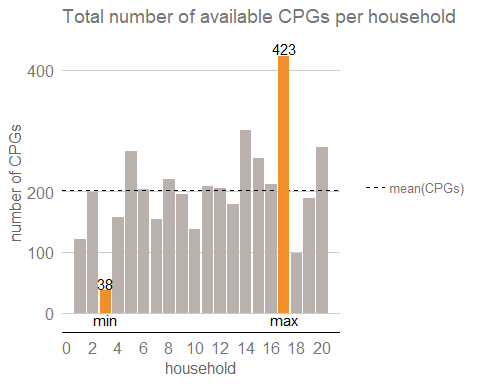
\includegraphics{test_files/figure-latex/unnamed-chunk-5-1} \end{center}

\subsubsection{List of items}\label{list-of-items}

\begin{table}

\caption{\label{tab:unnamed-chunk-6}List of consumer packaged goods}
\centering
\begin{tabular}[t]{>{\bfseries}l|l|>{\bfseries}l|l|>{\bfseries}l|l}
\hline
item & sub-cat & item & sub-cat & item & sub-cat\\
\hline
alioli & condiment & corianderPwd & spice & noodles & driedCarbs\\
\hline
alumFoil & disposableCover & corn & preparedCarbs & nuggets & meat\\
\hline
artichoke & veg & cornFlour & textureModifier & nuts & driedCarbs\\
\hline
asparagus & veg & courgette & veg & oil & cookingAgent\\
\hline
aubergine & veg & cream & dairy & oilFlavoured & cookingAgent\\
\hline
avocado & veg & cucumber & veg & onion & veg\\
\hline
bacon & meat & cumin & spice & oregano & spice\\
\hline
bag & disposableCover & curry & spice & oysterSauce & condiment\\
\hline
bagFreezer & disposableCover & disposables & disposableCover & panko & textureModifier\\
\hline
bakingPaper & disposableCover & dWashL & cleaningProduct & paprika & spice\\
\hline
bakingPwd & textureModifier & eggs & meat & pen & stationery\\
\hline
basil & veg & fennel & spice & pizza & readyToEat\\
\hline
basilPwd & spice & fishSauce & condiment & potatoes & veg\\
\hline
beans & preparedCarbs & fiveSpicesSeasoning & spice & prawns & meat\\
\hline
beanSprouts & veg & flour & textureModifier & rice & driedCarbs\\
\hline
beef & meat & food & food & riceQuinoa & driedCarbs\\
\hline
beer & beverage & frozenVegs & veg & rigatoni & driedCarbs\\
\hline
bellPepper & veg & garlic & veg & rosemary & spice\\
\hline
blackPepper & spice & garlicPwd & spice & salt & spice\\
\hline
bouillon & spice & ginger & veg & sausage & meat\\
\hline
bread & preparedCarbs & gloves & cleaningProducts & seasoning & spice\\
\hline
butter & dairy & goyaSeasoning & spice & seasoningChicken & spice\\
\hline
butternutSquash & veg & greenBeans & veg & soap & cleaningProduct\\
\hline
cabbage & veg & greenSnaps & veg & soda & beverage\\
\hline
cake & preparedCarbs & ham & meat & soySauce & condiment\\
\hline
cardamon & spice & hoisinSauce & condiment & spaghetti & driedCarbs\\
\hline
caribeanSpices & spice & hotSauce & condiment & spice\_ui & spice\\
\hline
carrots & veg & hummus & condiment & spinach & veg\\
\hline
cayenne & spice & hWashL & cleaningProduct & spirit & beverage\\
\hline
celery & veg & iceRocks & beverage & sponge & cleaningProduct\\
\hline
cheese & dairy & italianSpices & spice & springOnion & veg\\
\hline
chicken & meat & jam & condiment & sugar & spice\\
\hline
chickpeas & preparedCarbs & juice & beverage & sweetPotatoes & veg\\
\hline
chillies & veg & kale & veg & tahini & condiment\\
\hline
chilliesFlakes & spice & kitchenRoll & disposableCover & tea & beverage\\
\hline
chilliesPwd & spice & kiwi & fruit & thyme & veg\\
\hline
chineseGreens & veg & lard & cookingAgent & toiletPaper & cleaningProduct\\
\hline
chineseSpice & spice & leeks & veg & tomatoes & veg\\
\hline
chips & preparedCarbs & lemon & fruit & tomatoesProcessed & condiment\\
\hline
chives & spice & lettuce & veg & tomatoesSauce & condiment\\
\hline
chorizo & meat & lighter & cookingAgent & tortillas & preparedCarbs\\
\hline
cider & beverage & lime & fruit & turmeric & spice\\
\hline
cilantroBase & condiment & macarroni & driedCarbs & turnip & veg\\
\hline
cinamon & spice & mappleSyrup & condiment & vinegar & condiment\\
\hline
cleaningLiquid & cleaningProducts & marjoran & spice & water & cleaningProduct\\
\hline
clingFilm & disposableCover & masalaSpices & spice & whitePepper & spice\\
\hline
cloth & cleaningProducts & milk & dairy & wine & beverage\\
\hline
cocoa & spice & mincedMeat & meat & wipes & cleaningProduct\\
\hline
coconutCream & condiment & mint & veg & worcestershireSauce & condiment\\
\hline
coffee & beverage & mushrooms & veg & yogurt & dairy\\
\hline
coriander & veg & napkins & disposable &  & \\
\hline
\multicolumn{6}{l}{\textsuperscript{*} sub-cat = sub-category}\\
\end{tabular}
\end{table}

\begin{table}

\caption{\label{tab:unnamed-chunk-6}List of utensils}
\centering
\begin{tabular}[t]{>{\bfseries}l|l|>{\bfseries}l|l|>{\bfseries}l|l}
\hline
item & sub-cat & item & sub-cat & item & sub-cat\\
\hline
apron & protection & glassWine & contain & remoteControl & nonEssential\\
\hline
blender & prepare & grater & prepare & riceCooker & heat\\
\hline
bottle & contain & jar & contain & rSheet & informationAccess\\
\hline
bowl & contain & jarBlender & prepare & scale & measure\\
\hline
boxCondiments & contain & jarLid & cover & scissors & prepare\\
\hline
brush & clean & kettle & heat & sealingClips & store\\
\hline
bucket & contain & key & nonEssential & sinkDrainer & manipulate\\
\hline
canOpener & manipulate & knife & manipulate & smartAssistant & entertain\\
\hline
case & nonEssential & ladle & manipulate & smartWatch & informationAccess\\
\hline
charger & nonEssential & lid & cover & smasher & prepare\\
\hline
chopB & manipulate & lunchBag & contain & speaker & entertain\\
\hline
chopSticks & manipulate & measuringJar & measure & spoon & manipulate\\
\hline
clothes & nonEssential & measuringSpoon & measure & strainer & manipulate\\
\hline
coaster & hold & microwave & heat & tablet & entertain\\
\hline
coffeeMachine & heat & mixingBowl & contain & teaPot & heat\\
\hline
colander & manipulate & mop & clean & timer & measure\\
\hline
computer & informationAccess & mortar & prepare & toaster & heat\\
\hline
container & contain & ovenDish & contain & tongs & manipulate\\
\hline
cookingSpoon & manipulate & ovenGloves & hold & towel & clean\\
\hline
crusher & prepare & pan & heat & trashB & disposal\\
\hline
cup & contain & pastaServer & manipulate & tray & manipulate\\
\hline
cutlery & manipulate & peeler & prepare & vacuum & clean\\
\hline
dishTray & clean & phone & informationAccess & vaper & nonEssential\\
\hline
documents & informationAccess & plate & serve & vessel & nonEssential\\
\hline
dustBrush & clean & pot & heat & whisk & manipulate\\
\hline
dustPan & clean & processor & manipulate & wok & heat\\
\hline
fork & manipulate & radio & entertain & wristWatch & measure\\
\hline
glass & contain & rBook & informationAccess &  & \\
\hline
\multicolumn{6}{l}{\textsuperscript{*} sub-cat = sub-category}\\
\end{tabular}
\end{table}

\begin{table}

\caption{\label{tab:unnamed-chunk-6}List of environment}
\centering
\begin{tabular}[t]{>{\bfseries}l|l|>{\bfseries}l|l|>{\bfseries}l|l}
\hline
item & sub-cat & item & sub-cat & item & sub-cat\\
\hline
cpB & store & fireAlarm & nonEssential & plant & nonEssential\\
\hline
dishWasher & wash & freezer & preserve & stove & heat\\
\hline
dw & store & fridge & preserve & washingMachine & others\\
\hline
extractorFan & support & lightSwitch & support & window & others\\
\hline
faucet & clean & oven & heat &  & \\
\hline
\multicolumn{6}{l}{\textsuperscript{*} sub-cat = sub-category}\\
\end{tabular}
\end{table}

\subsubsection{Items by type}\label{items-by-type}

\subsubsection{Duration recipes}\label{duration-recipes}

\begin{table}

\caption{\label{tab:unnamed-chunk-8}Duration of recipes}
\centering
\begin{tabular}[t]{l|l|l}
\hline
session & regular & new\\
\hline
\rowcolor{gray!6}  1 & 36 & 61\\
\hline
2 & 76 & 81\\
\hline
\rowcolor{gray!6}  3 & 21 & 40\\
\hline
4 & 45 & 52\\
\hline
\rowcolor{gray!6}  5 & 41 & 90\\
\hline
6 & 45 & 90\\
\hline
\rowcolor{gray!6}  7 & 88 & 29\\
\hline
8 & 28 & 34\\
\hline
\rowcolor{gray!6}  9 & 68 & 78\\
\hline
10 & 39 & 111\\
\hline
\rowcolor{gray!6}  11 & 56 & 87\\
\hline
12 & 80 & 126\\
\hline
\rowcolor{gray!6}  13 & 42 & 53\\
\hline
14 & 73 & 58\\
\hline
\rowcolor{gray!6}  15 & 50 & 46\\
\hline
16 & 70 & 47\\
\hline
\rowcolor{gray!6}  17 & 113 & 90\\
\hline
18 & 44 & 80\\
\hline
\rowcolor{gray!6}  19 & 70 & 61\\
\hline
20 & 68 & 17\\
\hline
\end{tabular}
\end{table}

\begin{center}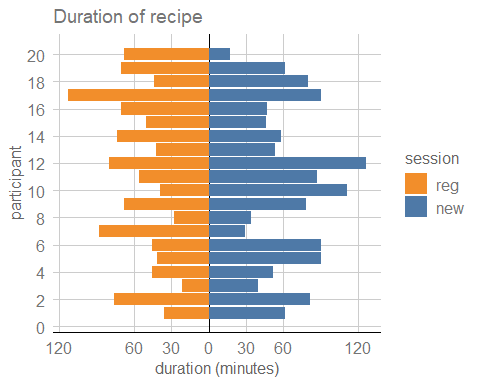
\includegraphics{test_files/figure-latex/unnamed-chunk-9-1} \end{center}

\begin{center}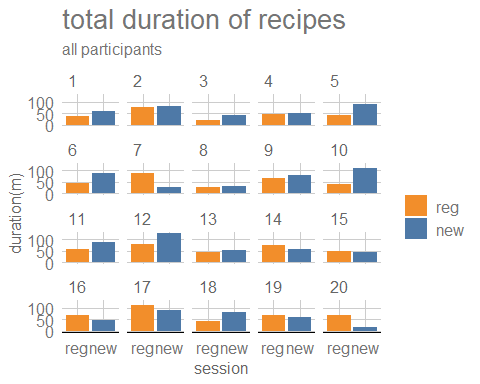
\includegraphics{test_files/figure-latex/unnamed-chunk-10-1} \end{center}

\subsubsection{Items used}\label{items-used}

The list of the items used

\begin{table}

\caption{\label{tab:unnamed-chunk-11}Total number of different items used}
\centering
\begin{tabular}[t]{c|c|c|c|c}
\hline
session & c & u & e & total\\
\hline
all & 970 & 1308 & 496 & 2774\\
\hline
regular & 465 & 567 & 237 & 1269\\
\hline
new & 505 & 741 & 259 & 1505\\
\hline
\multicolumn{5}{l}{\textsuperscript{*} c = CPGs, u = utensil, e = environment}\\
\end{tabular}
\end{table}

\subsubsection{Total number of different items
used}\label{total-number-of-different-items-used}

The total number of different items used were as follows:

\begin{table}

\caption{\label{tab:unnamed-chunk-12}Total number of different items used}
\centering
\begin{tabular}[t]{c|c|c|c|c}
\hline
session & c & u & e & total\\
\hline
all & 970 & 1308 & 496 & 2774\\
\hline
regular & 465 & 567 & 237 & 1269\\
\hline
new & 505 & 741 & 259 & 1505\\
\hline
\multicolumn{5}{l}{\textsuperscript{*} c = CPGs, u = utensil, e = environment}\\
\end{tabular}
\end{table}

\end{document}
